\chapter{Výběry a jejich rozdělení}

\section{Výběr a populace}

\subsection{Definice základních pojmů}

\begin{definition}[Cílová populace]
Soubor všech prvků, které jsou předmětem našeho zájmu, nazýváme cílovou populací.
\end{definition}

\begin{example}
V astronomii můžeme být cílovou populací soubor všech hvězd ve vesmíru a předmětem zájmu jejich hmotnost. V letectví mohou cílovou skupinu představovat všechny vyrobené letouny daného typu, kde zkoumáme životnost jejich draku.
\end{example}

V praxi bývá velmi často nemožné nebo nežádoucí zjišťovat danou vlastnost na celé cílové populaci\footnote{Hvězd ve vesmíru je příliš mnoho na to, abychom je mohli všechny jednotlivě zkoumat. Testování odolnosti draku všech letounů by vedlo k jejich zničení, a proto postrádá smysl.}. Řešením je tak vybrat část populace a tu následně podrobit zkoumání - zjištění pak zobecníme na celou populaci.

Jestliže lze na každý prvek cílové populace nahlížet jako na náhodnou veličinu s danou pravděpodobnostní funkcí\footnote{Na hmotnost hvězdy a na životnost draku letadla lze zcela jistě pohlížet jako na náhodnou veličinu.}, pak lze pro tuto populaci definovat náhodný výběr.

\begin{definition}[Náhodný výběr]
Nechť mají náhodné veličiny $X_1, ..., X_n$ sdruženou pravděpodobnostní funkci, pro kterou platí
\begin{equation*}
f_{X_1, ..., X_n}(x_1, ..., x_n) = f(x_1) \cdots f(x_n)
\end{equation*}
kde $f(\cdot)$ představuje pravděpodobnostní funkci, která je shodná pro všechna $X_i$. Pak definujeme $X_1, ..., X_n$ jako náhodný výběr velikosti $n$ z populace s pravděpodobnostní funkcí $f(\cdot)$.
\end{definition}

Náhodná veličina $X_i$ reprezentuje hodnotu $i$-tého prvku výběru. Po té, co je výběr zanalyzován, nabývá náhodná veličina $X_i$ konkrétní hodnoty $x_i$. Proto se někdy pod pojmem náhodný výběr rozumí $x_1, ..., x_n$ namísto $X_1, ..., X_n$.

Velmi často není možné pořídit náhodný výběr z cílové populace. V těchto případech pak cílovou populaci nahrazujeme tzv. výběrovou populací.

\begin{definition}[Výběrová populace]
Nechť $X_1, ..., X_n$ je náhodný výběr z populace s pravděpodobnostní funkcí $f(\cdot)$. Tuto populaci pak nazýváme výběrovou populací.
\end{definition}

Závěry na základě náhodného výběru lze vztáhnout pouze na výběrovou populaci, nikoliv na cílovou populaci. Jedinou vyjímkou je situace, kdy je cílová populace zároveň výběrovou populací.

\begin{example}
Uvažujme marketingovou studii, jejímž cílem je zkoumat nákupní zvyky domácností dané země. Pokud budeme náhodný vzorek domácností vybírat z určitého regionu, pak tento region bude představovat naši výběrovou populaci. Naší cílovou populací však budou dománosti celé země. Je také zřejmé, že nákupní zvyklosti domácností se mohou mezi jednotlivými regiony lišit, a proto zobecnění z jednoho regionu na celou zemi může být problematické.
\end{example}

V následujícím textu budeme někdy používat označení ``populace $f(\cdot)$'', čímž budeme mít na mysli populaci, jejíž jednotlivé prvky mají pravděpodobnostní rozdělení $f(\cdot)$. Pokud budeme používat slovo populace bez přívlastku, budeme tím mít na mysli vždy výběrovou populaci.

\subsection{Rozdělení výběru}

\begin{definition}[Rozdělení výběru]
Nechť $X_1, ..., X_n$ označují náhodný výběr velikosti $n$. Pak rozdělení výběru $X_1, ..., X_n$ je dáno sdruženým rozdělením náhodných veličin $X_1, ..., X_n$.
\end{definition}

\begin{definition}
Jestliže $X_1, ..., X_n$ představují náhodný výběr z populace $f(\cdot)$, pak pravděpodobnostní rozdělení tohoto výběru je dáno sdruženou pravděpodobnostní funkcí
\begin{equation*}
f_{X_1, ..., X_n}(x_1, ..., x_n)(x_1, ..., x_n) = f(x_1) \cdots f(x_n)
\end{equation*}
\end{definition}

\begin{example}
Uvažujme populaci, jejíž prvky sledují Bernoulliho rozdělení. Sdružená pravděpodobnostní funkce dvou prvkového náhodného výběru je tedy
\begin{equation*}
f_{X_1, X_2}(x_1, x_2) = f(x_1)f(x_2) = p^{x_1 + x_2}q^{2 - x_1 - x_2}I_{(0, 1)}(x_1)I_{(0, 1)}(x_2)
\end{equation*}
\end{example}

Pravděpodobnostní funkce $f_{X_1, X_2}(x_1, x_2)$ z výše uvedeného příkladu definuje rozdělení uspořádaného výběru. Záleží tedy nejen na typu a počtu realizací, ale také na jejich uspořádání.

Dále je zřejmé, že naše definice náhodného výběru automaticky zavrhuje výběr bez vracení z konečné populace, protože jednotlivé ``tahy'' nejsou vzájemně nezávislé.

\subsection{Statistiky a výběrové momenty}

\begin{definition}[Statistika]
Statistika je funkcí pozorovatelných náhodných veličin, a je tak sama o sobě pozorovatelnou náhodnou veličinou, která neobsahuje žádné neznámé parametry. 
\end{definition}

\begin{example}
Jestliže $X_1, ..., X_n$ představuje náhodný výběr z populace $f(\cdot, \theta)$, pak, za předpokladu, že $X_1, ..., X_n$ jsou pozorovatelné, jsou
\begin{equation*}
\overline{X}_n = \frac{1}{n} \sum_{i = 1}^n X_i
\end{equation*}
a
\begin{equation*}
\frac{1}{2}(\min(X_1, ..., X_n) + \max(X_1, ..., X_n))
\end{equation*}
statistikami. Pokud $f(x, \theta) = \phi_{\theta, 1}(x)$, kde $\theta$ je neznámý parametr, pak $\overline{X}_n - \theta$ není statistikou, právě proto, že závisí na neznámé $\theta$. 
\end{example}

V následující definici představíme jedny z  nejdůležitějších statistik, tzv. výběrové momenty.

\begin{definition}[Výběrové momenty]
Nechť $X_1, ..., X_n$ představuje náhodný výběr z populace $f(\cdot)$. Pak je $r$-tý obecný výběrový moment definován jako
\begin{equation*}
M'_r = \frac{1}{n} \sum_{i = 1}^n X_i^r
\end{equation*}
Jestliže $r = 1$, pak získáme výběrový moment obvykle označovaný jako $\overline{X}$ popř. jako $\overline{X}_n$.
\begin{equation*}
\overline{X}_n = \frac{1}{n} \sum_{i = 1}^n X_i
\end{equation*}
Podobně je $r$-tý centrální výběrový moment definován jako
\begin{equation*}
M_r = \frac{1}{n} \sum_{i = 1}^n \left(X_i - \overline{X}_n \right)^r
\end{equation*}
\end{definition}

\begin{theorem}
Nechť $X_1, ..., X_n$ představují náhodný výběr z populace $f(\cdot)$. Očekávaná hodnota $r$-tého výběrového momentu $M'_r$ je rovna $r$-tému momentu populace $\mu'_r$ za předpokladu existence $\mu'_r$. 
\begin{equation*}
E[M'_r] = \mu'_r
\end{equation*}
Dále také platí
\begin{equation*}
D[M'_r] = \frac{1}{n}\left(E[X^{2r}] - E[X^r]^2 \right) = \frac{1}{n} [\mu'_{2r} - (\mu'_r)^2]
\end{equation*}
za předpokladu existence $\mu'_{2r}$.
\end{theorem}

\begin{proof}
\begin{gather*}
E[M'_r] = E \left[\frac{1}{n} \sum_{i = 1}^n X_i^r \right] = \frac{1}{n} E \left[\sum_{i = 1}^n X_i^r \right] = \frac{1}{n} \sum_{i = 1}^n E[X_i^r] = \frac{1}{n} \sum_{i = 1}^n \mu'_r = \mu'_r
\end{gather*}
\begin{gather*}
D[M'_r] = D\left[\frac{1}{n} \sum_{i = 1}^n X_i^r \right] = \left(\frac{1}{n} \right)^2 D \left[ \sum_{i = 1}^n X_i^r \right] = \left(\frac{1}{n} \right)^2 \sum_{i = 1}^n \left(E[X_i^{2r}] - E[X_i^r]^2 \right)\\
= \frac{1}{n} \left(E[X^2r] - E[X^r]^2 \right) = \frac{1}{n}\left(\mu'_{2r} - (\mu'_r)^2 \right)
\end{gather*}
\end{proof}

\begin{corollary}
Nechť $X_1, ..., X_n$ představuje náhodný výběr z populace $f(\cdot)$ a $\overline{X}_n = \frac{1}{n} \sum_{i = 1}^n X_i$ představuje výběrovou střední hodnotu. Pak platí
\begin{gather*}
E[\overline{X}_n] = \mu\\
D[\overline{X}_n] = \frac{1}{n} \sigma^2
\end{gather*}
kde $\mu$ a $\sigma^2$ jsou střední hodnota a rozptyl pravděpodobnostního rozdělení $f(\cdot)$.
\end{corollary}

\begin{definition}[Výběrový rozptyl]
Nechť $X_1, ..., X_n$ představují náhodný výběr z populace $f(\cdot)$. Výběrový rozptyl je pak definován jako
\begin{equation*}
S_n^2 = \frac{1}{n - 1} \sum_{i = 1}^n (X_i - \overline{X})^2
\end{equation*}
pro $n > 1$.
\end{definition}

Výběrový rozptyl je definován jako $S_n^2 = \frac{1}{n - 1} \sum_{i = 1}^n (X_i - \overline{X})^2$ namísto druhého výběrového momentu $M_2 = \frac{1}{n} \sum_{i = 1}^n (X_i - \overline{X})^2$, protože střední hodnota $S_n^2$ je rovna rozptylu populace.

\begin{corollary}
\begin{equation*}
S_n^2 = \frac{1}{2n(n-1)} \sum_{i = 1}^n \sum_{j = 1}^n (X_i - X_j)^2
\end{equation*}
\end{corollary}

\begin{proof}
\begin{gather*}
\frac{1}{2n(n - 1)} \sum_{i = 1}^n \sum_{j = 1}^n (X_i - X_j)^2 = \frac{1}{2n(n - 1)}\sum_{i = 1}^n \left(nX_i^2 - 2 X_i \sum_{j = 1}^n X_j + \sum_{j = 1}^n X_j^2 \right)\\
= \frac{1}{2n(n - 1)} \sum_{i = 1}^n \left(nX_i^2 - 2n \overline{X}X_i + n \overline{X^2} \right) = \frac{1}{2(n-1)}\left(n \overline{X^2} - 2 \overline{X}^2 + n \overline{X^2} \right)\\
= \frac{1}{n - 1}(n\overline{X^2} - \overline{X}^2) = \frac{1}{n - 1}nD[X] = \frac{1}{n - 1}\sum_{i = 1}^n (X_i - \overline{X})^2
\end{gather*}
\end{proof}

\begin{theorem}
Nechť $X_1, ..., X_n$ představuje náhodný výběr z populace $f(\cdot)$ a nechť $S_n^2 = \frac{1}{n - 1} \sum_{i = 1}^n (X_i - \overline{X})^2$. Pak platí
\begin{gather*}
E[S_n^2] = \sigma^2\\
D[S_n^2] = \frac{1}{n}\left(\mu_4 - \frac{n - 3}{n - 1}\sigma^4 \right)
\end{gather*}
pro $n > 1$.
\end{theorem}

\begin{proof}
Nejprve dokažme tvrzení o střední hodnotě výběrového rozptylu. Připomeňme, že platí $\sigma^2 = E[(X - \mu)^2]$ a $\mu_r = E[(X - \mu)^r]$. Jádro důkazu spočívá v identitě
\begin{equation*}
\sum_{i = 1}^n (X_i - \mu)^2 = \sum_{i = 1}^n (X_i - \overline{X})^2 + n (\overline{X} - \mu)^2
\end{equation*}
Platnost této identity lze dokázat následujícím způsobem.
\begin{gather*}
\sum(X_i - \mu)^2 = \sum(X_i - \overline{X} + \overline{X} - \mu)^2 = \sum [(X_i - \overline{X}) + (\overline{X} - \mu)]^2]\\
= \sum[(X_i - \overline{X})^2 + 2(X_i - \overline{X})(\overline{X} - \mu) + (\overline{X} - \mu)^2]\\
= \sum(X_i - \overline{X})^2 + 2(\overline{X} - \mu)\sum(X_i - \overline{X}) + n (\overline{X} - \mu)^2
= \sum(X_i - \overline{X})^2 + n(\overline{X} - \mu)^2
\end{gather*}
S využitím této identity pak lze odvodit
\begin{gather*}
E[S_n^2] = E \left[\frac{1}{n - 1} \sum (X_i - \overline{X})^2 \right] = \frac{1}{n - 1} E \left[\sum_{i = 1}^n (X_i - \mu)^2 - n(\overline{X} - \mu)^2 \right]\\
\frac{1}{n - 1} \Big\{\sum_{i = 1}^n E[(X_i - \mu)^2] - n E[(\overline{X} - \mu)^2] \Big\} = \frac{1}{n - 1}\Big\{\sum_{i = 1}^n \sigma^2 - n D[\overline{X}] \Big\}\\
= \frac{1}{n - 1}\left(n \sigma^2 - n \frac{\sigma^2}{n} \right) = \sigma^2
\end{gather*}

Důkaz rozptylu $S_n^2$ lze provést s využitím výše odvozené identity a vztahu
\begin{equation*}
\overline{X} - \mu = \frac{1}{n} \sum X_i - \frac{1}{n} n \mu = \frac{1}{n} \sum X_i - \frac{1}{n} \sum \mu = \frac{1}{n} \sum (X_i - \mu)
\end{equation*}
Nicméně odvození je poměrně zdlouhavé, a proto jej vynecháme.
\end{proof}

\section{Výběrová střední hodnota}

\subsection{Střední hodnota a rozptyl}

\begin{theorem}
Nechť $X_1, ..., X_n$ představuje náhodný výběr z populace $f(\cdot)$ se střední hodnotou $\mu$ a konečným rozptylem $\sigma^2$. Definujme $\overline{X} = \frac{1}{n} \sum_{i = 1}^n X_i$. Pak platí
\begin{equation*}
E[\overline{X}] = \mu_{\overline{x}} = \mu ~~~ D[\overline{X}] = \sigma_{\overline{X}^2} = \frac{1}{n} \sigma^2
\end{equation*}
\end{theorem}
Tento teorém je v podstatě pouze reformulací tvrzení (6.1).

Výběrová střední hodnota $\overline{X}$ má charakter náhodné veličiny. Pokud bychom ji použili jako odhad pro $\mu$, pak platí, že její střední hodnota odpovídá hledané střední hodnotě populace $\mu$ a že její rozptyl klesá s rostoucí velikostí náhodného výběru. Tímto se dostáváme k zákonu velkých čísel.

\subsection{Zákon velkých čísel}

Označme střední hodnotu náhodné veličiny $X$ s pravděpodobnostní funkcí $f(\cdot)$ jako $\mu$. Předpokládejme, že předmětem našeho zájmu je odhad $\mu$.

Na $\mu$ lze nahlížet jako na průměr nekonečného počtu hodnot náhodné veličiny $X$. Je zřejmé, že reálném životě nejsme schopni průměrovat nekonečný počet hodnot, a proto musíme informace o $\mu$ získat na základě náhodného výběru z populace $f(\cdot)$ velikosti $n$. To nám umožňuje tzv. slabý zákon velkých čísel.

\begin{theorem}[Slabý zákon velkých čísel]
Nechť $f(\cdot)$ představuje pravděpodobnostní funkci se střední hodnotou $\mu$ a rozptylem $\sigma^2$. Dále nechť $\overline{X}_n$ představuje střední hodnotu náhodného výběru velikosti $n$ z populace $f(\cdot)$. Uvažujme dvě čísla $\epsilon > 0$ a $0 < \delta < 1$. Jestliže $n$ je přirozené číslo takové, že $n > \frac{\sigma^2}{\epsilon^2} \delta$, pak
\begin{equation*}
P[-\epsilon < \overline{X}_n - \mu < \epsilon] \ge 1 - \delta
\end{equation*}  
\end{theorem}  

\begin{proof}
Dle Chebyshevovy nerovnosti platí
\begin{equation*}
P[g(X) \ge k] \le \frac{E[g(X)]}{k}
\end{equation*}
pro každé $k > 0$, libovolnou náhodnou veličinu $X$ a nezápornou funkci $g(\cdot)$. Tato nerovnost je ekvivalentní s
\begin{equation*}
P[g(X) < k] \ge 1 - \frac{E[g(X)]}{k}
\end{equation*}
Nechť $g(X) = (\overline{X}_n - \mu)^2$ a $k = \epsilon^2$. Pak
\begin{gather*}
P[-\epsilon < \overline{X}_n - \mu < \epsilon] = P[|\overline{X}_n - \mu| < \epsilon]\\
= P[|\overline{X}_n - \mu|^2 < \epsilon^2] \ge 1 - \frac{E[(\overline{X}_n - \mu)^2]}{\epsilon^2}\\
= 1 - \frac{\frac{1}{n}\sigma^2}{\epsilon^2} \ge 1 - \delta
\end{gather*}
pro $\delta > \frac{\sigma^2}{n \epsilon^2}$ popř. $n > \frac{\sigma^2}{\epsilon^2} \delta$.
\end{proof}

\begin{example}
Uvažujme pravděpodobnostní rozdělení s neznámou střední hodnotou a rozptylem 1. Jak velký musí být náhodný výběr, aby se jeho střední hodnota $\overline{X}_n$ nacházela ve vzdálenosti 0.5 od střední hodnoty populace s pravděpodobnostní alespoň 0.95?

Dosaďme $\sigma^2 = 1, \epsilon = 0.5$ a $\delta = 0.05$. Minimální velikost $n$ náhodného výběru je dána vztahem
\begin{equation*}
n > \frac{\sigma^2}{\delta \epsilon} = \frac{1}{0.05 \cdot (0.5)^2} = 80
\end{equation*} 
\end{example}

\subsection{Centrální limitní věta}

S centrální limitní větou jsme se již seznámili v předchozí kapitole. Nyní se k ní opět vrátíme a doplníme ji o důkaz.

\begin{theorem}[Centrální limitní věta]
Nechť $f(\cdot)$ představuje pravděpodobnostní funkci se střední hodnotou $\mu$ a konečným rozptylem $\sigma^2$. Dále nechť $\overline{X}_n$ představuje střední hodnotu náhodného výběru velikosti $n$ z populace $f(\cdot)$. Definujme náhodnou veličinu
\begin{equation*}
Z_n = \frac{\overline{X}_n - E[\overline{X}_n]}{\sqrt{D[\overline{X}_n]}} = \frac{\overline{X}_n - \mu}{\frac{\sigma}{\sqrt{n}}}
\end{equation*}
Pravděpodobnostní rozdělení náhodné veličiny $Z_n$ se limitně blíží normovanému normálnímu rozdělení s tím, jak se $n$ blíží nekonečnu.
\end{theorem}
Nejpozoruhodnější skutečností na centrální limitní větě je, že platí pro všechny pravděpodobnostní funkce $f(\cdot)$. Centrální limitní věta implikuje, že pravděpodobnostní funkce výběrové střední hodnoty $\overline{X}_n$ se asymptoticky blíží normálnímu rozdělení se střední hodnotou $\mu$ a rozptylem $\frac{\sigma^2}{n}$ bez ohledu na výchozí pravděpodobnosntí funkci $f(\cdot)$.

\begin{proof}
Centrální limitní větu nebudeme dokazovat v její obecné formě. Zaměříme se na situaci, kdy $f(\cdot)$ má momentovou funkci. Připomeňme, že momentová funkce normovaného normálního rozdělení je $m(t) = e^{\frac{1}{2}t^2}$. Pro momentovou funkci $m_{Z_n}(t)$ náhodné veličiny $Z_n$ se pak pokusíme dokázat, že se asymptoticky blíží k $m(t)$. 

Momentová funkce $m_{Z_n}(t)$ je definována jako
\begin{gather*}
m_{Z_n}(t) = E[e^{tZ_n}] = E\left[e^{t\frac{\overline{X} - \mu}{\sigma / \sqrt{n}}} \right] = E\left[e^{\frac{t}{n}\sum \frac{X_i - \mu}{\sigma / \sqrt{n}}} \right]\\
= E\left[\prod_{i = 1}^n e^{\frac{t}{n} \frac{X_i - \mu}{\sigma / \sqrt{n}}} \right] = \prod_{i = 1}^n E \left[e^{\frac{t}{\sqrt{n}}\frac{X_i - \mu}{\sigma}} \right]
\end{gather*}
kde jsme v posledním kroku využili nezávislosti náhodných veličin $X_1, ..., X_n$. Definujme $Y_i = \frac{X_i - \mu}{\sigma}$. Momentová funkce náhodné veličiny $Y_i$ je nezávislá na $i$, protože všechna $Y_i$ mají shodné pravděpodobnostní rozdělení. Proto namísto $m_{Y_i}(t)$ budeme používat značení $m_Y(t)$. Platí
\begin{gather*}
\prod_{i = 1}^n E \left[e^{\frac{t}{\sqrt{n}} \frac{X_i - \mu}{\sigma}} \right] = \prod_{i = 1}^n e^{\frac{t}{\sqrt{n}} Y_i}\\
= \prod_{i = 1}^n m_Y\left(\frac{t}{\sqrt{n}}\right) = \left[m_Y\left(\frac{t}{\sqrt{n}}\right)\right]^n
\end{gather*}
a proto
\begin{equation*}
m_{Z_n(t)} = \left[m_Y \left(\frac{t}{\sqrt{n}}\right)\right]^n
\end{equation*}
$r$-tou derivací $m_Y(t/\sqrt{n})$ v bodě $t = 0$ získáme $r$-tý moment okolo střední hodnoty pro pravděpodobnostní funkci $f(\cdot)$ vydělený členem $(\sigma \sqrt{n})^r$. S pomocí Taylorova rozvoje tak lze $m_Y(t/\sqrt{n})$ vyjádřit jako
\begin{equation*}
m_Y\left(\frac{t}{\sqrt{n}}\right) = 1 + \frac{\mu_1}{\sigma}\frac{t}{\sqrt{n}}+\frac{1}{2!}\frac{\mu_2}{\sigma^2} \left(\frac{t}{\sqrt{n}}\right)^2 + \frac{1}{3!} \frac{\mu_3}{\sigma^3} \left(\frac{t}{\sqrt{n}}\right)^3 + \cdots
\end{equation*}
a protože $\mu_1 = 0$ a $\mu_2 = \sigma^2$, lze tento výraz dále upravit na
\begin{equation*}
m_Y\left(\frac{t}{\sqrt{n}}\right) = 1 + \frac{1}{n}\left(\frac{1}{2}t^2 + \frac{1}{3! \sqrt{n}}\frac{\mu_3}{\sigma^3} t^3 + \frac{1}{4!n}\frac{\mu_4}{\sigma^4}t^4 + \cdots \right)
\end{equation*}
Protože $\lim_{n \rightarrow \infty}\left(1 + \frac{u}{n} \right)^n = e^{\frac{1}{2}t^2}$, kde
\begin{equation*}
u = \frac{1}{2}t^2 + \frac{1}{3! \sqrt{n}}\frac{\mu_3}{\sigma^3} t^3 + \frac{1}{4!n}\frac{\mu_4}{\sigma^4}t^4 + \cdots
\end{equation*}
představuje výraz v závorkách ve výše uvedené rovnici. Tím se dostáváme k $\lim_{n \rightarrow \infty} m_{Z_n}(t) = e^{\frac{1}{2}t^2}$. Proto má $Z_n$ v limitě stejnou momentovou funkci jako normalizované normální rozdělení. Připomeňme, že pokud mají dvě náhodné veličiny shodnou momentovou funkci, pak sledují shodné pravděpodobnostní rozdělení.
\end{proof}

Je zřejmé, že míra aproximace záleží na velikosti náhodného výběru a konkrétní pravděpodobnostní funkci $f(\cdot)$. Situace pro $f(x) = e^{-x}I_{(0, \infty)}(x)$ pro $n = 1, 3, 10$ je ilustrována obrázkem (\ref{asymptotic-normal}), kde souvislá čára představuje skutečné rozdělení a přerušovaná čára pak aproximaci normálním rozdělením.

\begin{figure}[htp]
\centering
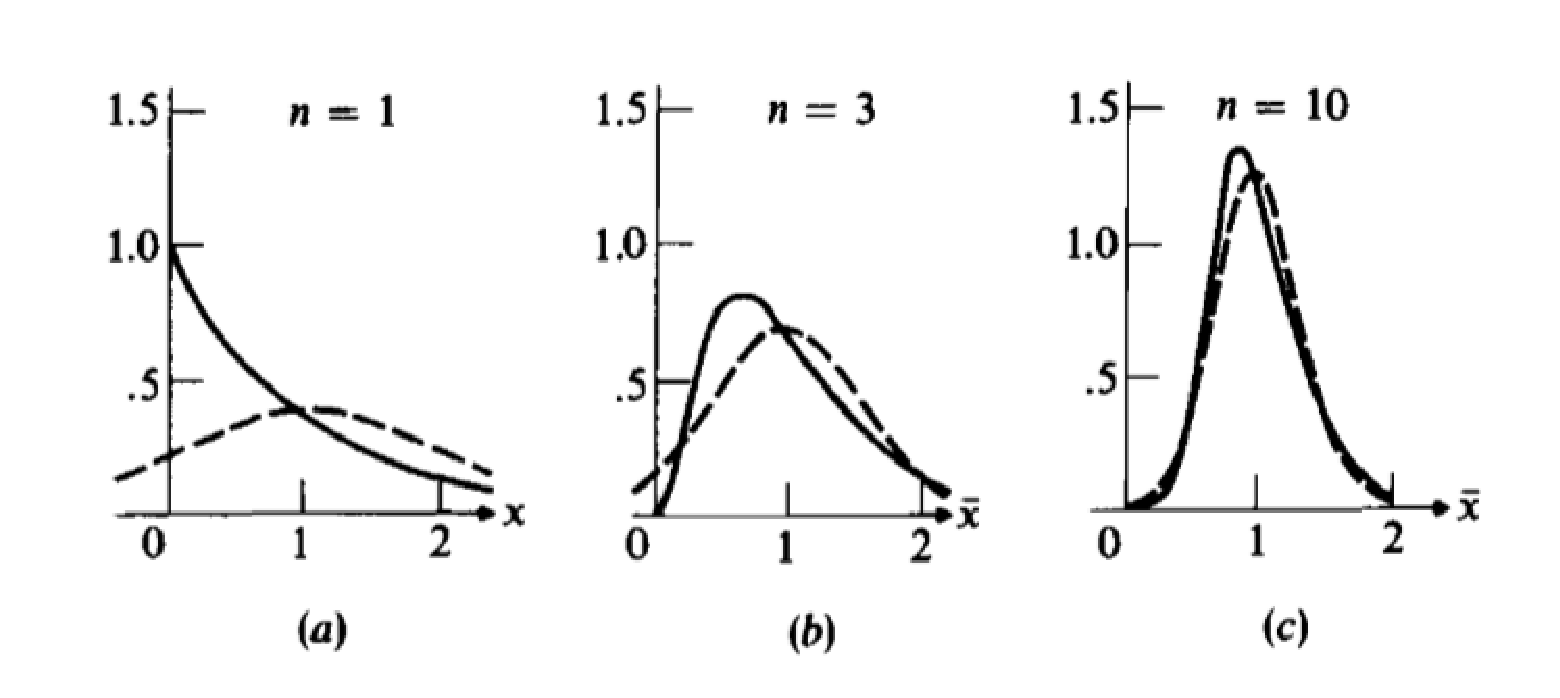
\includegraphics[scale = 0.5]{pictures/asymptotic_normal.eps}
\caption{Konvergence k normálnímu rozdělení}
\label{asymptotic-normal}
\end{figure}

Jak je z obrázku (\ref{asymptotic-normal}) patrné, aproximace se poměrně rychle zlepšuje s rostoucí velikostí náhodného výběru. Obrázek se zaměřuje na konvergenci v okolí střední hodnoty $\mu$. Co z něj však patrné není, je konvergence v okolí chvostů, kde je míra konvergence výrazně pomalejší.

Následující kapitoly se zaměřují na pravděpodobnostní rozdělení střední hodnoty výběru pro konkrétní pravděpodobnostní funkci $f(\cdot)$.

\subsection{Bernoulliho rozdělení}

Jestliže $X_1, ..., X_n$ představují náhodný výběr z Bernoulliho rozdělení, lze nalézt přesnou formu pravděpodobnostního rozdělení náhodné veličiny $\overline{X}_n$. Pravděpodobnostní funkce, ze které provádíme náhodný výběr, má formu
\begin{equation*}
f(x) = p^x(1 - p)^{1 - x}I_{(0, 1)}(x)
\end{equation*}
Z příkladu (5.7) víme, že $\sum_{i = 1}^n X_i$ sleduje binomické rozdělení.
\begin{equation*}
P \left[\sum_{i = 1}^n X_i = k \right] = \binom{n}{k}p^k q^{n - k}I_{\{0, 1, ..., n\}}(k)
\end{equation*}
Proto je pravděpodobnostní rozdělení $\overline{X}_n$ dáno vztahem
\begin{equation*}
P \left[\overline{X}_n = \frac{k}{n} \right] = \binom{n}{k}p^k q^{n - k}~~~\textit{pro}~ k = 0, 1, ..., n 
\end{equation*}
Proto náhodná veličina $\overline{X}_n$ nabývá v případě Bernoulliho rozdělení hodnot $0, 1/n, ..., 1$ s pravděpodobnostmi $\binom{n}{0}p^0 q^n, \binom{n}{1}p^1 q^{n - 1}, \binom{n}{2}p^2 q^{n - 2}, ..., \binom{n}{n}p^n q^0$.

\subsection{Poissonovo rozdělení}

Jestliže $X_1, ..., X_n$ představují náhodný výběr z Poissonova rozdělení se střední hodnotou $\lambda$, pak z příkladu (5.8) vyplývá, že $\sum_{i = 1}^n X_i$ sleduje Poissonovo rozdělení s parametrem $n \lambda$. Proto platí
\begin{equation*}
P \left[\overline{X}_n = \frac{k}{n} \right] = P\left[\sum_{i = 1}^n X_i = k \right] = \frac{e^{-n \lambda}(n \lambda)^k}{k!}~~~\textit{pro}~k = 0, 1, 2, ...
\end{equation*}

\subsection{Exponenciální rozdělení}

Nechť $X_1, ..., X_n$ představují náhodný výběr z exponenciálního rozdělení
\begin{equation*}
f(x) = \theta e^{-\theta x}I_{(0, \infty)}(x)
\end{equation*}
Z příkladu (5.9) víme, že $\sum_{i = 1}^n$ má gamma rozdělení s parametry $n$ a $\theta$. Proto platí
\begin{equation*}
f_{\sum X_i}(z) = \frac{1}{\Gamma(n)}z^{n - 1} \theta^n e^{-\theta z} I_{(0, \infty)}(z)
\end{equation*}
neboli
\begin{equation*}
P[\sum X_i \le y] = \int_0^y \frac{1}{\Gamma(n)}z^{n - 1} \theta^n e^{- \theta z}dz ~~~ \textit{pro}~ y > 0
\end{equation*}
což lze upravit do tvaru
\begin{gather*}
P \left[\overline{X}_n \le \frac{y}{n} \right] = \int_0^y \frac{1}{\Gamma(n)}z^{n - 1} \theta^n e^{- \theta z} dz\\
P[\overline{X}_n \le x] = \int_0^{nx} \frac{1}{ \Gamma(n)}z^{n - 1} \theta^n e^{-\theta z} dz = \int_0^x \frac{1}{\Gamma(n)}(nu)^{n-1}\theta^n e^{-n \theta u}n du
\end{gather*}
To znamená, že $\overline{X}_m$ sleduje gamma rozdělení s parametry $n$ a $n \theta$.

\subsection{Uniformní rozdělení}

Nechť $X_1, ..., X_n$ představuje náhodný výběr z uniformního rozdělení nad intervalem $(0, 1]$. Pravděpodobnostní funkce náhodné veličiny $\overline{X}_n$ je dána vztahem
\begin{gather*}
f_{\overline{X}_n}(x) = \sum_{k = 0}^{n - 1} \frac{n}{(n - 1)!} \Big[(nx)^{n - 1} - \binom{n}{1}(nx - 1)^{n - 1} + \binom{n}{2}(nx - 2)^{n - 1} - \cdots \\
+ (-1)^k \binom{n}{k}(nx - k)^{n - 1} \Big]I_{(k/n, (k + 1)/n]}(x)
\end{gather*}

Obecné odvození výše uvedeného vztahu je založené na indukci a konvoluci a je poněkud zdlouhavé, a proto jej vynecháme.

\subsection{Cauchyho rozdělení}

Nechť $X_1, ..., X_n$ představuje náhodný výběr z Cauchyho rozdělení a
\begin{equation*}
f(x) = \frac{1}{\pi \beta \{1 + [(x - \alpha)/\beta]^2\}}
\end{equation*}
Potom sleduje $\overline{X}_n$ stejné Cauchyho rozdělení pro libovolné $n$. To znamená, že střední hodnota výběru má stejné pravděpodobostní rozdělení jako libovolný prvek tohoto výběru.

Momentová funkce Cauchyho rozdělení neexistuje a důkaz pomocí indukce a konjunkce vede ke složitým integrálům. Nejjednodušším způsobem je tak důkaz pomocí tzv. charakteristické funkce, která je zobecněním momentové funkce. Charakteristická funkce má oproti momentové funkci tu výhodu, že vždy existuje. Samotný důkaz se pak opírá o skutečnost, že součin charakteristických funkcí nezávislých náhodných veličin se shodným pravděpodobnostním rozdělením je charakteristickou funkcí součtu těchto náhodných veličin.

\section{Výběr z normálního rozdělení}

\subsection{Střední hodnota výběru}

\begin{theorem}
Nechť $\overline{X}_n$ označuje střední hodnotu náhodného výběru velikosti $n$ z normálního rozdělení se střední hodnotou $\mu$ a rozptylem $\sigma^2$. Pak má $\overline{X}_n$ normální rozdělení se střední hodnotou $\mu$ a rozptylem $\sigma^2/n$.
\end{theorem}

\begin{proof}
\begin{gather*}
m_{\overline{X}_n}(t) = E[e^{t \overline{X}_n}] = E\left[e^{\frac{t \sum X_i}{n}} \right] = E\left[\prod_{i = 1}^n e^{\frac{t X_i}{n}} \right] = \prod_{i = 1}^n E\left[e^{\frac{t X_i}{n}} \right]\\
=\prod_{i = 1}^n m_i \left(\frac{t}{n}\right) = \prod_{i = 1}^n e^{\frac{\mu t}{n} + \frac{1}{2} \left(\frac{\sigma t}{n}\right)^2} = e^{\mu t + \frac{\frac{1}{2}(\sigma t)^2}{n}}
\end{gather*}
$e^{\mu t + \frac{\frac{1}{2}(\sigma t)^2}{n}}$ je momentová funkce normálního rozdělení se střední hodnotou $\mu$ a rozptylem $\sigma^2 / n$, čímž uzavíráme důkaz.
\end{proof}

\subsection{Chi-kvadrát rozdělení}

\begin{definition}[Chi-kvadrát rozdělení]
Jestliže je $X$ náhodná veličina s pravděpodobnostní funkcí
\begin{equation*}
f_X(x) = \frac{1}{\Gamma(k/2)} \left(\frac{1}{2}\right)^{\frac{k}{2}} x^{\frac{k}{2} - 1}e^{-\frac{1}{2}x}I_{(0, \infty)}(x) 
\end{equation*}
pak tato náhodná veličina sleduje chi-kvadrát rozdělení s $k$ stupni volnosti, kde $k$ je přirozené číslo.
\end{definition}

\begin{corollary}
Chi-kvadrát rozdělení je specifickým případem gamma rozdělení s parametry $r = \frac{k}{2}$ a $\lambda = \frac{1}{2}$. Proto pro náhodnou veličinu $X$, která sleduje chi-kvadrát rozdělení, platí
\begin{gather*}
E[X] = k\\
D[X] = 2k\\
m_X(t) = \left(\frac{1}{1 - 2t}\right)^{\frac{k}{2}}, ~~~ \textit{pro} ~ t < \frac{1}{2}
\end{gather*}
\end{corollary}

\begin{theorem}
Jestliže náhodné veličiny $X_i$ pro $i = 1, 2, ..., k$ jsou nezávislé a sledují normální rozdělení se střední hodnotou $\mu_i$ a rozptyle $\sigma_i^2$, pak náhodná veličina
\begin{equation*}
U = \sum_{i = 1}^k \left(\frac{X_i - \mu_i}{\sigma_i}\right)^2
\end{equation*}
sleduje chi-kvadrát rozdělení s $k$ stupni volnosti.
\end{theorem}

\begin{proof}
Definujme $Z_i = \frac{X_i - \mu_i}{\sigma_i}$. Pak $Z_i$ sleduje normalizované normální rozdělení. Její momentová funkce je definována jako
\begin{equation*}
m_U(t) = E[e^{tU}] = E[e^{t \sum Z_i^2}] = E \left[\prod_{i = 1}^n e^{t Z_i^2} \right] = \prod_{i = 1}^k E \left[ e^{t Z_i^2} \right]
\end{equation*}
Zároveň však platí
\begin{gather*}
E \left[ e^{t Z_i^2} \right] = \int_{-\infty}^{\infty}e^{t z^2} \left(\frac{1}{\sqrt{2 \pi}} \right) e^{-\frac{1}{2}z^2} dz = \int_{-\infty}^{\infty} \frac{1}{\sqrt{2 \pi}} e^{-\frac{1}{2}(1 - 2t)z^2}dz\\
= \frac{1}{\sqrt{1 - 2t}} \int_{-\infty}^{\infty} \frac{\sqrt{1 - 2t}}{\sqrt{2 \pi}} e^{-\frac{1}{2}(1 - 2t)z^2}dz = \frac{1}{\sqrt{1 - 2t}}
\end{gather*}
pro $t < \frac{1}{2}$, kde je poslední integrál roven jedné, protože představuje plochu pod křivkou normálního rozdělení s rozptylem $\frac{1}{\sqrt{1 - 2t}}$.
\begin{equation*}
\prod_{i = 1}^k E \left[e^{t Z_i^2} \right] = \prod_{i = 1}^k \frac{1}{\sqrt{1 - 2t}} = \left(\frac{1}{1 - 2t}\right)^{\frac{k}{2}}
\end{equation*}
tak představuje momentovou funkci chi-kvadrát rozdělení s $k$ stupni volnosti.
\end{proof}

\begin{corollary}
Jestliže $X_1, ..., X_n$ představuje náhodný výběr z normálního rozdělení se střední hodnotou $\mu$ a rozptylem $\sigma^2$, pak $U = \sum_{i = 1}^n \frac{(X_i - \mu)^2}{\sigma^2}$ sleduje chi-kvadrát rozdělení s $n$ stupni volnosti.
\end{corollary}

Jestliže je $\mu$ nebo $\sigma^2$ neznámé, pak není náhodná veličina $U$ statická. Jestliže je však $\mu$ známé a $\sigma^2$ neznámé, lze odhadnout $\sigma^2$ pomocí $\frac{1}{n} \sum_{i = 1}^n (X_i - \mu)^2$ a rozdělení $\frac{1}{n} \sum_{i = 1}^n (X_i - \mu)^2$ odvodit na základě výše uvedeného tvrzení. To je možné, protože platí
\begin{equation*}
E \left[\frac{1}{n} \sum_{i = 1}^n (X_i - \mu)^2 \right] = \frac{1}{n} \sum_{i = 1}^n E[(X_i - \mu)^2] = \frac{1}{n} \sum_{i = 1}^n \sigma^2 = \sigma^2
\end{equation*}

\begin{theorem}
Jestliže $Z_1, ..., Z_n$ představují náhodný výběr z normovaného normálního rozdělení, pak
\begin{enumerate}
\item $\overline{Z}$ sleduje normální rozdělení s nulovou střední hodnotou a rozptylem $\frac{1}{n}$.
\item $\overline{Z}$ a $\sum_{i = 1}^n(Z_i - \overline{Z})^2$ jsou nezávislé.
\item $\sum_{i = 1}^n (Z_i - \overline{Z})^2$ sleduje chi-kvadrát rozdělení s $n - 1$ stupni volnosti.
\end{enumerate}
\end{theorem}

\begin{proof}
Bod (1) vychází z věty (6.6).

Bod (2) dokážeme pro $n = 2$. Jestliže $n = 2$, pak $\overline{Z} = \frac{Z_1 + Z_2}{2}$ a
\begin{gather*}
\sum (Z_i - \overline{Z})^2 = \left(Z_1 - \frac{Z_1 + Z_2}{2} \right)^2 + \left(Z_2 - \frac{Z_1 + Z_2}{2} \right)^2\\
= \frac{(Z_1 - Z_2)^2}{4} + \frac{(Z_2 - Z_1)^2}{4} = \frac{(Z_2 - Z_1)^2}{2}
\end{gather*}
takže $\overline{Z}$ je funkcí $Z_1 + Z_2$ a $\sum (Z_i - \overline{Z})^2$ je funkcí $Z_2 - Z_1$. Abychom prokázali, že $\overline{Z}$ a $\sum (Z_i - \overline{Z})^2$ jsou nezávislé, stačí prokázat nezávislost $Z_1 + Z_2$ a $Z_2 - Z_1$. Pro jejich momentové funkce platí
\begin{equation*}
m_{Z_1 + Z_2}(t_1) = E\left[e^{t_1(Z_1 + Z_2)} \right] = E[e^{t_1 Z_1} e^{t_1 Z_2}] = E\left[e^{t_1 Z_1}\right]E\left[e^{t_1 Z_2}\right] = e^{\frac{1}{2} t_1^2}e^{\frac{1}{2} t_1 t_1^2} = e^{t_1^2}
\end{equation*}
a podobně
\begin{equation*}
m_{Z_2 - Z_1}(t_2) = e^{t_2^2}
\end{equation*}
Dále také platí
\begin{gather*}
m_{Z_1 + Z_2, Z_2 - Z_1}(t_1, t_2) = E\left[e^{t_1 (Z_1 + Z_2) + t_2 (Z_2 - Z_1)} \right] = E\left[e^{(t_1 - t_2)Z_1}e^{(t_1 + t_2)Z_2} \right]\\
= E\left[e^{(t_1 - t_2)Z_1}\right]E\left[e^{(t_1 + t_2)Z_2}\right] = e^{\frac{1}{2}(t_1 - t_2)^2}e^{\frac{1}{2}(t_1 + t_2)^2} = e^{t_1^2}e^{t_2^2} = m_{Z_1 + Z_2}(t_1)m_{Z_2 - Z_1}(t_2)
\end{gather*}
což znamená, že $Z_1 + Z_2$ a $Z_2 - Z_1$ jsou nezávislé.

Abychom dokázali bod (3) využijeme nezávislosti $\overline{Z}$ a $\sum_{i = 1}^n(Z_i - \overline{Z})^2$, což jsme prokázali výše. Všimněme si, že
\begin{gather*}
\sum Z_i^2 = \sum (Z_i - \overline{Z} + \overline{Z})^2 = \sum(Z_i - \overline{Z})^2 + 2 \overline{Z} \sum (Z_i - \overline{Z}) + \sum \overline{Z}^2\\
= \sum (Z_i - \overline{Z})^2 + n \overline{Z}^2
\end{gather*}
Proto platí
\begin{equation*}
m_{\sum Z_i^2}(t) = m_{\sum(Z_i - \overline{Z})^2}(t)m_{n \overline{Z}^2}(t)
\end{equation*}
což implikuje
\begin{equation*}
m_{\sum (Z_i - \overline{Z})^2(t)} = \frac{m_{\sum Z_i^2}(t)}{m_{n \overline{Z}^2}(t)} = \frac{\left(\frac{1}{1 - 2t}\right)^{\frac{n}{2}}}{\left(\frac{1}{1 - 2t}\right)^{\frac{1}{2}}} = \left( \frac{1}{1 - 2t} \right)^{\frac{n - 1}{2}}
\end{equation*}
pro $t < \frac{1}{2}$. Protože náhodná veličina $\sqrt{n}\overline{Z}$ sleduje normované normální rozdělení, sleduje $n \overline{Z}^2$ chi-kvadrát rozdělení s jedním stupněm volnosti, čímž jsme dokázali, že momentová funkce náhodné veličiny $\sum (Z_i - \overline{Z})^2$ je momentovou funkcí chi-kvadrát rozdělení s $n - 1$ stupni volnosti.
\end{proof}

\begin{theorem}
Předchozí věta předpokládála, že náhodný výběr pochází z normovaného normálního rozdělení. Pokud bychom namísto toho předpokládali náhodný výběr z normálního rozdělení se střední hodnotou $\mu$ a rozptylem $\sigma^2$, pak $Z_i = \frac{X_i - \mu}{\sigma}$. Výše uvedená věta se tak modifikuje do tvaru
\begin{enumerate}
\item $\overline{Z} = \frac{1}{n}\sum \frac{X_i - \mu}{\sigma} = \frac{\overline{X} - \mu}{\sigma}$ sleduje normální rozdělení nulovou střední hodnotou a rozptylem $\frac{1}{n}$.
\item $\overline{Z} = \frac{\overline{X} - \mu}{\sigma}$ a $\sum (Z_i - \overline{Z})^2 = \sum \left(\frac{X_i - \mu}{\sigma} - \frac{\overline{X} - \mu}{\sigma}\right)^2$ jsou nezávislé, což implikuje nezávislost mezi $\overline{X}$ a $\sum(X_i - \overline{X})^2$.
\item $\sum (Z_i - \overline{Z})^2 = \sum \frac{(X_i - \overline{X})^2}{\sigma^2}$ sleduje chi-kvadrát rozdělení s $n - 1$ stupni volnosti.
\end{enumerate}
\end{theorem}

\begin{corollary}
Jestliže $S_n^2 = \frac{1}{n - 1}\sum_{i = 1}^n(X_i - \overline{X})^2$ představuje rozptyl náhodného výběru z normálního rozdělení se střední hodnotou $\mu$ a rozptylem $\sigma^2$, pak
\begin{equation*}
U = \frac{(n - 1) S_n^2}{\sigma^2}
\end{equation*}
sleduje chi-kvadrát rozdělení s $n - 1$ stupni volnosti.
\end{corollary}
Protože $S_n^2$ je lineární funkcí náhodné veličiny $U$, lze pravděpodobnostní rozdělení $S_n^2$ získat z pravděpodobnostního rozdělení $U$.
\begin{equation*}
f_{S_n^2}(y) = \left(\frac{n - 1}{2 \sigma^2}\right)^{\frac{n - 1}{2}} \frac{1}{\Gamma \left(\frac{n - 1}{2}\right)}y^{\frac{n - 3}{2}}e^{-\frac{(n - 1)y}{2 \sigma^2}}I_{(0, \infty)}(y)
\end{equation*}

Pojem ``stupně volnosti'' lze chápat jako počet nezávislých členů v součtu. Např. součet ve větě (6.7) má $k$ nezávislých členů, zatímco součet v bodě (3) věty (6.8) má pouze $n - 1$ nezávislých členů. To proto, že vztah $\sum(Z_i - \overline{Z}) = 0$ umožňuje výpočet $Z_i - \overline{Z}$ pro libovolné $i$ za předpokladu znalosti zbývajících $n - 1$ členů.

\subsection{F rozdělení}

Uvažujme dvě nezávislé náhodné veličiny $U$ a $V$, které sledují chi-kvadrát rozdělení s $m$ resp. $n$ stupni volnosti. Jejich sdružená pravděpodobnostní funkce je pak dána rovnicí
\begin{equation*}
f_{U,V}(u,v) = \frac{1}{\Gamma(m/2)\Gamma(n/2)2^{(m + n)/2}}u^{\frac{m-2}{2}}v^{\frac{n - 2}{2}}e^{-\frac{1}{2}(u + v)}I_{(0, \infty)}(u)I_{(0, \infty)}(v)
\end{equation*}
Předmětem našeho zájmu je pravděpodobnostní rozdělení podílu
\begin{equation*}
X = \frac{U/m}{V/n}
\end{equation*}
V prvním kroku provedeme transformaci $X = \frac{U/m}{V/n}$ a $Y = V$, nalezneme sdruženou pravděpodobnostní funkci $X$ a $Y$ a následně integrací získáme marginální pravděpodobnostní funkci náhodné veličiny $X$.

Jakobián výše uvedené transformace je $\frac{m}{n}y$, proto
\begin{equation*}
f_{X,Y}(x,y) = \frac{m}{n}y \frac{1}{\Gamma(m/2)\Gamma(n/2)2^{(m + n)/2}}\left(\frac{m}{n}xy\right)^{\frac{m-2}{2}}y^{\frac{n - 2}{2}}e^{-\frac{1}{2}\left(\frac{m}{n}xy + y \right)}
\end{equation*}
Následnou integrací pak získáme
\begin{gather*}
f_X(x) = \int_0^{\infty} f_{X,Y}(x,y)dy\\
= \frac{1}{\Gamma(m/2)\Gamma(n/2)2^{(m + n)/2}}\left(\frac{m}{n}\right)^{\frac{m}{2}}x^{\frac{m - 2}{2}} \int_0^{\infty} y^{\frac{m + n - 2}{2}}e^{-\frac{1}{2}\left(\frac{m}{n}x + 1 \right)y}dy\\
= \frac{\Gamma((m+2)/2)}{\Gamma(m/2)\Gamma(n/2)}\left(\frac{m}{n}\right)^{\frac{m}{2}}\frac{x^{\frac{m-2}{2}}}{\left(1 + \frac{m}{n}x \right)^{(m + n)/2}}I_{(0, \infty)}(x)
\end{gather*}

\begin{definition}[F rozdělení]
Jestliže náhodná veličina $X$ má pravděpodobostní funkci
\begin{equation*}
f(x) = \frac{\Gamma((m+2)/2)}{\Gamma(m/2)\Gamma(n/2)}\left(\frac{m}{n}\right)^{\frac{m}{2}}\frac{x^{\frac{m-2}{2}}}{\left(1 + \frac{m}{n}x \right)^{(m + n)/2}}I_{(0, \infty)}(x)
\end{equation*}
pak tato náhodná veličina sleduje F rozdělení s $m$ a $n$ stupni volnosti.
\end{definition}

Pořadí, ve které jsou stupně volnosti uváděny, je důležité, protože F rozdělení není symetrické v těchto parametrech. Počet stupňů volnosti $m$ v podílu $\frac{m}{n}$ výše uvedené pravděpodobnostní funkce je vždy uváděn jako první.

\begin{theorem}
Nechť $U$ a $V$ jsou nezávislé náhodné veličiny, které sledují chi-kvadrát rozdělení s $m$ resp. $n$ stupni volnosti. Pak náhodná veličina
\begin{equation*}
X = \frac{U/m}{V/n}
\end{equation*}
sleduje F rozdělení s $m$ a $n$ stupni volnosti.
\end{theorem}

\begin{corollary}
Nechť $X_1, ..., X_{m+1}$ představuje náhodný výběr velikosti $m+1$ z normálního rozdělení se střední hodnotou $\mu_X$ a rozptylem $\sigma^2$. Nechť $Y_1, ..., Y_{n+1}$ představuje náhodný výběr velikosti $n+1$ z normálního rozdělení se střední hodnotou $\mu_Y$ a rozptylem $\sigma^2$. Nechť jsou oba náhodné výběry nezávislé. Pak
\begin{equation*}
\frac{1}{\sigma^2}\sum_{i = 1}^{m+1}(X_i - \overline{X})^2
\end{equation*}
sleduje chi-kvadrát rozdělení s $m$ stupni volnosti a
\begin{equation*}
\frac{1}{\sigma^2}\sum_{i = 1}^{n+1}(Y_i - \overline{Y})^2
\end{equation*}
sleduje chi-kvadrát rozdělení s $n$ stupni volnosti. Proto
\begin{equation*}
\frac{\sum(X_i - \overline{X})^2/m}{\sum(Y_j - \overline{Y})/n}
\end{equation*}
sleduje F rozdělení s $m$ a $n$ stupni volnosti.
\end{corollary}

\begin{theorem}
Jestliže náhodná veličina $X$ sleduje F distribuci s $m$ a $n$ stupni volnosti, pak
\begin{gather*}
E[X] = \frac{n}{n - 2} ~~~ \textit{pro} ~ n > 2\\
D[X] = \frac{2 n ^2 (m + n - 2)}{m(n - 2)^2(n - 4)} ~~~ \textit{pro} ~ n > 4
\end{gather*}
\end{theorem}

\begin{proof}
Dokažme tvrzení o střední hodnotě.
\begin{equation*}
E[X] = E \left[\frac{U/m}{V/n}\right] = \frac{n}{m}E[U]E\left[\frac{1}{V}\right]
\end{equation*}
Protože $U$ sleduje chi-kvadrát rozdělení s $m$ stupni volnosti, platí $E[U] = m$. Pro $E \left[\frac{1}{V} \right]$ je situace o něco složitější.
\begin{gather*}
E \left[\frac{1}{V}\right] = \frac{1}{\Gamma(n/2)}\left(\frac{1}{2}\right)^{\frac{n}{2}}\int_0^{\infty} \frac{1}{v} v^{\frac{n-2}{2}}e^{-\frac{1}{2}v}dv\\
= \frac{1}{\Gamma(n/2)}\left(\frac{1}{2}\right)^{\frac{n}{2}}\int_0^{\infty} v^{\frac{n - 4}{2}}e^{-\frac{1}{2}v}dv\\
= \frac{\Gamma((n - 2) / 2)}{\Gamma(n / 2)}\left(\frac{1}{2}\right)^{\frac{n}{2}}\left(\frac{1}{2}\right)^{-\frac{n-2}{2}} = \frac{1}{n - 2}
\end{gather*}
Proto platí
\begin{equation*}
E[X] = \left(\frac{n}{m}\right)E[U]E\left[\frac{1}{V}\right] = \frac{n}{m}\frac{m}{n - 2} = \frac{n}{n - 2}
\end{equation*}
Tvrzení o střední hodnotě lze dokázat analogicky.
\end{proof}

Jestliže $X$ sleduje F rozdělení s $m$ a $n$ stupni volnosti, pak $1/X$ sleduje F rozdělení s $n$ a $m$ stupni volnosti. Tento vztah umožňuje definovat tabulky tohoto pravděpodobnostního rozdělení pouze pro horní polovinu kvantilů. Platí totiž
\begin{equation*}
p = P[X \le \xi_p] = P \left[\frac{1}{X} \ge \frac{1}{\xi} \right] = P \left[Y \ge \frac{1}{\xi_p} \right] = 1 - P\left[Y \le \frac{1}{\xi_p} \right]
\end{equation*}
což znamená $1 - p = P[Y \le \xi'_{1 - p}]$, a proto $\xi'_{1 - p} = \frac{1}{\xi_p}$.

Jestliže $X$ sleduje F rozdělení s $m$ a $n$ stupni volnosti, pak
\begin{equation*}
W = \frac{m \frac{X}{n}}{1 + m \frac{X}{n}}
\end{equation*}
sleduje beta rozdělení s parametry $a = m/2$ a $b = n/2$.
 
\subsection{Studentovo rozdělení}

\begin{theorem}[Studentovo rozdělení]
Uvažujme náhodnou veličinu $Z$, která sleduje normované normální rozdělení, a náhodnou veličinu $U$, která sleduje chi-kvadrát rozdělení s $k$ stupni volnosti. Jestliže jsou $Z$ a $U$ nezávislé, pak náhodná veličina $\frac{Z}{\sqrt{U/k}}$ sleduje studentovo rozdělení s $k$ stupni volnosti.
\end{theorem}

Sdružená pravděpodobnostní funkce náhodných veličin $Z$ a $U$ je
\begin{equation*}
f_{Z,U}(z,u) = \frac{1}{\sqrt{2 \pi}} \frac{1}{\Gamma(k/2)} \left( \frac{1}{2} \right)^{\frac{k}{2}}u^{\frac{k}{2} - 1}e^{-\frac{1}{2}u}e^{-\frac{1}{2}z^2}I_{(0, \infty)}(u)
\end{equation*}
Jestliže použijeme transformaci $X = \frac{Z}{\sqrt{U/k}}$ a $Y = U$, pak je Jakobián roven $\sqrt{\frac{y}{k}}$, a proto
\begin{equation*}
f_{X,Y}(x,y) = \sqrt{\frac{y}{k}}\frac{1}{\sqrt{2 \pi}}\frac{1}{\Gamma(k/2)}\left(\frac{1}{2}\right)^{\frac{k}{2}}y^{\frac{k}{2} - 1}e^{-\frac{1}{2}y}e^{-\frac{1}{2}\frac{x^2y}{k}}I_{(0, \infty)}(y)
\end{equation*}
Následnou integrací pak získáme marginální pravděpodobnostní funkci náhodné veličiny $X$.
\begin{gather*}
f_X(x) = \int_{-\infty}^{\infty} f_{X,Y}(x,y)dy = \frac{1}{\sqrt{2 k \pi}} \frac{1}{\Gamma(k/2)} \left(\frac{1}{2} \right)^{\frac{k}{2}} \int_0^{\infty}y^{\frac{k}{2} - 1 + \frac{1}{2}}e^{-\frac{1}{2}\left(1 + \frac{x^2}{k}\right)y}dy\\
= \frac{\Gamma \left((k + 1)/2\right)}{\Gamma(k/2)} \frac{1}{\sqrt{k \pi}} \frac{1}{\left(1 + \frac{x^2}{k} \right)^{\frac{k + 1}{2}}}
\end{gather*}

\begin{definition}[Studentovo rozdělení]
Jestliže pravděpodobnostní rozdělení náhodné veličiny $X$ má tvar
\begin{equation*}
 f_X(x) = \frac{\Gamma \left((k + 1)/2\right)}{\Gamma(k/2)} \frac{1}{\sqrt{k \pi}} \frac{1}{\left(1 + \frac{x^2}{k} \right)^{\frac{k + 1}{2}}}
\end{equation*}
pak tato náhodná veličina sleduje studentovo rozdělení s $k$ stupni volnosti.
\end{definition}

\begin{corollary}
Jestliže $X_1, ..., X_n$ představuje náhodný výběr z normálního rozdělení se střední hodnotou $\mu$ a rozptylem $\sigma^2$, pak $Z = \frac{\overline{X} - \mu}{\sigma / \sqrt{n}}$ sleduje normalizované normální rozdělení a $U = \frac{1}{\sigma^2} \sum (X_i - \overline{X})^2$ sleduje chi-kvadrát rozdělení s $n - 1$ stupni volnosti. Nezávislost $Z$ a $U$ vyplývá z věty (6.8), a proto
\begin{equation*}
\frac{\frac{\overline{X} - \mu}{\sigma / \sqrt{n}}}{\sqrt{\frac{1}{\sigma^2} \sum \frac{(X_i - \overline{X})^2}{n - 1}}} = \frac{\sqrt{n(n - 1)}(\overline{X} - \mu)}{\sqrt{\sum (X_i - \overline{X})^2}}
\end{equation*}
sleduje studentovo rozdělení s $n - 1$ stupni volnosti.
\end{corollary}

V případě jednoho stupně volnosti se studentovo rozdělení zredukuje na Cauchyho rozdělení. Naopak s rostoucím počtem stupňů volnosti se studentovo rozdělení blíží normalizovanému normálnímu rozdělení. Dále platí, že druhá mocnina studentova rozdělení s $k$ stupni volnosti odpovídá F rozdělení s jedním a $k$ stupni volnosti.

\begin{definition}
Jestliže náhodná veličina $X$ sleduje studentovo rozdělení s $k$ stupni volnosti, pak
\begin{gather*}
E[X] = 0 ~~~ \textit{pro} ~ k > 1\\
D[X] = \frac{k}{k - 2} ~~~ \textit{pro} ~ k > 2
\end{gather*}
\end{definition}

\begin{proof}
Postup tohoto důkazu je podobný důkazu (6.8). Připomeňme, že $X = \frac{Z}{\sqrt{U / k}}$, kde $Z$ a $U$ jsou nezávislé. To implikuje
\begin{equation*}
E[X] = E\left[\frac{Z}{\sqrt{U/k}}\right] = E[Z]\sqrt{k}E\left[\frac{1}{\sqrt{U}} \right] = 0 \cdot \sqrt{k}E\left[\frac{1}{\sqrt{U}} \right] = 0
\end{equation*}
a
\begin{equation*}
E[X^2] = E\left[\frac{Z^2}{U/k}\right] = E[Z^2] \cdot k \cdot E\left[\frac{1}{U} \right] = 1 \cdot k \cdot \frac{1}{k - 2} = \frac{k}{k - 2}
\end{equation*}
Rozptyl náhodné veličiny $X$ je tedy
\begin{equation*}
D[X] = E[X^2] - E[X]^2 = \frac{k}{k - 2}
\end{equation*}
\end{proof}

\section{Pořadové statistiky}

\begin{definition}[Pořadové statistiky]
Nechť $X_1, ..., X_2$ představuje náhodný výběr velikosti $n$ z kumulativní distribuční funkce $F(\cdot)$. Pak $Y_1 \le Y_2 \le \cdots \le Y_n$, kde $Y_i$ jsou vzestupně seřazená $X_i$, nazýváme pořadovou statistikou náhodného výběru $X_1, ..., X_n$.
\end{definition}

Z výše uvedené definice je zřejmé, že jednotlivá $Y_i$ nejsou nezávislá, protože je-li $Y_j \ge y$, pak také $Y_{j + 1} \ge y$.

\begin{theorem}
Nechť $Y_1 \le Y_2 \le \cdots \le Y_n$ představuje pořadovou statistiku z kumulativní distribuční funkce $F(\cdot)$. Marginální kumulativní distribuční funkce náhodné veličiny $Y_{\alpha}$, kde $\alpha = 1, 2, ..., n$, je dána
\begin{equation*}
F_{Y_{\alpha}}(y) = \sum_{j = \alpha}^n \binom{n}{j}[F(y)]^j [1 - F(y)]^{n - j}
\end{equation*}
\end{theorem}

\begin{proof}
Pro fixní $y$ definujme $Z_i = I_{(-\infty, y]}(X_i)$. Je zřejmé, že $\sum_{i = 1}^n Z_i$ je rovno počtu náhodných veličin $X_i$, pro která platí $X_i \le y$. Platí
\begin{equation*}
F_{Y_{\alpha}} = P[Y_{\alpha} \le y] = P\left[\sum_i Z_i \ge \alpha \right] = \sum_{j = \alpha}^n \binom{n}{j}[F(y)]^j [1 - F(y)]^{n - j}
\end{equation*}
Klíčovým krokem důkazu je ekvivalence jevů $\{Y_a \le y\}$ a $\big\{\sum Z_i \ge \alpha \big\}$. Jestliže je totiž $\alpha$-tá pořadová statistika menší nebo rovna $y$, pak je počet $X_i$, která jsou menší nebo rovna $y$, větší nebo roven $\alpha$ a naopak.
\end{proof}

\begin{corollary}
\begin{gather*}
F_{Y_n}(y) = \sum_{j = n}^n \binom{n}{j}F[(y)]^j [1 - F(y)]^{n - j} = [F(y)]^n\\
F_{Y_1}(y) = \binom{n}{j}[F(y)]^j[1 - F(y)]^{n - j} = 1 - [1 - F(y)]^n
\end{gather*}
\end{corollary}

Po zbytek této kapitoly budeme předpokládat, že náhodný vzorek $X_1, ..., X_n$ pochází ze spojitého rozdělení.

Pravděpodobnostní funkci $f_{Y_{\alpha}}(y)$ lze získat derivací výše odovozené kumulativní distribuční funkce.
\begin{gather*}
f_{Y_{\alpha}}(y) = \lim_{\Delta y \rightarrow 0} \frac{F_{Y_{\alpha}}(y + \Delta y) - F_{Y_{\alpha}}(y)}{\Delta y} = \lim_{\Delta y \rightarrow 0} \frac{P[y < Y_{\alpha} \le y + \Delta y]}{\Delta y}\\
= \lim_{\Delta y \rightarrow 0} \frac{P[(\alpha - 1) ~ X_i \le y, \textit{jedno} ~ X_i ~ \textit{v} ~ (y, y + \Delta y], (n - \alpha) ~ X_i > y + \Delta y}{\Delta y}\\
= \lim_{\Delta y \rightarrow 0} \frac{n!}{(\alpha - 1)!1!(n - \alpha!)}\frac{[F(y)]^{\alpha - 1}[F(y + \Delta y) - F(y)][1 - F(y + \Delta y)]^{n - a}}{\Delta y}\\
= \frac{n!}{(\alpha - 1)!(n - \alpha)!}[F(y)]^{\alpha - 1}[1 - F(y)]^{n - \alpha}f(y)
\end{gather*}
Podobně lze odvodit sdruženou pravděpodobnostní funkci náhodných veličin $Y_{\alpha}$ a $Y_{\beta}$, kde $1 \le \alpha < \beta \le n$.
\begin{gather*}
f_{Y_{\alpha}, Y_{\beta}}(x,y) \Delta x \Delta y \approx P[x < Y_{\alpha} \le x + \Delta x, y < Y_{\beta} \le y + \Delta y]\\
\approx P[(\alpha - 1) ~ X_i \le x, \textit{jedno} ~ X_i ~ \textit{v}~ (x, x + \Delta x],\\
(\beta - \alpha - 1) ~ X_i ~ \textit{v} ~ (x + \Delta x, y], \textit{jedno} ~ X_i ~ \textit{v} ~ (y, y + \Delta y], (n - \beta) ~ X_i > y + \Delta y]\\
\approx \frac{n!}{(\alpha - 1)! 1! (\beta - \alpha - 1)! 1! (n - \beta)!}\\
\times [F(X)]^{\alpha - 1}[F(y) - F(x + \Delta x)]^{\beta - \alpha - 1}[1 - F(y + \Delta y)]^{n - \beta} f(x) \Delta x f(y) \Delta y
\end{gather*}
Proto pro $x < y$ platí
\begin{equation*}
f_{Y_{\alpha}. Y_{\beta}}(x,y) =
\frac{n!}{(\alpha - 1)!(\beta - \alpha - 1)!(n - \beta)!}[F(x)]^{\alpha - 1}[F(y) - F(x)]^{\beta - \alpha - 1}[1 - F(y)]^{n - \beta} f(x) f(y)
\end{equation*}
Sdruženou pravděpodobnostní funkci $f_{Y_1, ..., Y_n}(y1, ..., y_n)$ pak lze odvodit jako
\begin{gather*}
f_{Y_1, ..., Y_n}(y1, ..., y_n) = \lim_{\Delta y_i \rightarrow 0} \frac{1}{\prod_{i = 1}^n \Delta y_i} P[y_1 < Y_1 \le y_1 + \Delta y_1, ..., y_n < Y_n \le y_n + \Delta y_n]\\
= \lim_{\Delta y_i \rightarrow 0} \frac{1}{\prod_{i = 1}^n \Delta y_i}P[\textit{jedno}~X_i ~ \textit{v} ~ (y_1, y_1 + \Delta y_1), ..., \textit{jedno}~X_i ~ \textit{v} ~ (y_n, y_n + \Delta y_n)]\\
= \lim_{\Delta y_i \rightarrow 0} \frac{n!}{\prod_{i = 1}^n \Delta y_i} [F(y_1 + \Delta y_1) - F(y_1)], \cdots ,[F(y_n + \Delta y_n) - F(y_n)]\\
= n! f(y_1) \cdots f(y_n)
\end{gather*}
pro $y_1 < y_2 < \cdots < y_n$.

\begin{theorem}
Nechť $X_1, ..., X_n$ představuje náhodný výběr z populace $f(\cdot)$ s kumulativní distribuční funkcí $F(\cdot)$. Dále nechť $Y_1 \le Y_2 \le \cdots \le Y_n$ představuje odpovídající pořadovou statistiku. Pak platí
\begin{gather*}
f_{Y_{\alpha}}(y) = \frac{n!}{(\alpha - 1)!(n - \alpha)!}[F(y)]^{\alpha - 1}[1 - F(y)]^{n - \alpha}f(y)\\
f_{Y_{\alpha}, Y_{\beta}}(x,y) = \frac{n!}{(\alpha - 1)!(n - \alpha)!}[F(y)]^{\alpha - 1}[F(y) - F(x)]^{\beta - \alpha - 1}[1 - F(y)]^{n - \beta}f(x)f(y)\\
f_{Y_1, ..., Y_n}(y_1, ..., y_n) = n!f(y_1) \cdots f(y_n)
\end{gather*}
\end{theorem}

\subsection{Rozdělení funkcí pořadových statistik}

Jednou z možných funkcí pořadových statistik je jejich aritmetický průměr $\frac{1}{n} \sum_{j = 1}^n Y_j$. Nicméně $\frac{1}{n} \sum_{j = 1}^n Y_j = \frac{1}{n} \sum_{i = 1}^n X_i$, což je střední hodnota náhodného výběru. Proto se zaměříme na jiné fukce pořadových statistik.

\begin{definition}[Výběrový medián, rozpětí výběru a střed výběru]
Nechť $Y_1 \le \cdots \le Y_n$ označuje pořadové statistiky náhodného výběru $X_1, ..., X_n$ z populace $f(\cdot)$. Výběrový medián je definován jako prostřední statistika, je-li $n$ liché popř. jako průměr dvou prostředních statistik, je-li $n$ sudé. Rozpětí výběru je definováno jako $Y_n - Y_1$ a střed výběru jako $\frac{Y_1 + Y_n}{2}$.
\end{definition}

Pokusme se odvodit sdruženou pravděpodobnostní funkci výběrového mediánu a rozpětí výběru. Jestliže je $n$ liché, pak je pravděpodobnostní funkce výběrového mediánu dána první rovnicí věty (6.14). Jestliže je $n$ sudé a výběrový medián je tak definován jako $\frac{Y_{n/2} + Y_{n/2 + 1}}{2}$ pak je jeho pravděpodobnostní funkce dána druhou rovnicí věty (6.14). Dle třetí rovnice věty (6.14) platí
\begin{equation*}
f_{Y_1, Y_n}(x,y) = n (n - 1)[F(y) - F(x)]^n-2 f(x)f(y)
\end{equation*}
Jestliže použijeme transformaci $R = Y_n - Y_1$ a $\frac{Y_1 + Y_n}{2}$ popř. $r = y - x$ a $t = \frac{x + y}{2}$, získáme $x = t - \frac{r}{2}$ a $y = t + \frac{r}{2}$ a Jakobián je tak roven
\begin{equation*}
J =
\begin{vmatrix}
\frac{\partial x}{\partial r} & \frac{\partial x}{\partial t}\\
\frac{\partial y}{\partial r} & \frac{\partial y}{\partial t}
\end{vmatrix}
=
\begin{vmatrix}
-\frac{1}{2} & 1\\
\frac{1}{2} & 1
\end{vmatrix}
= -1
\end{equation*}
čímž se dostáváme následující větě.

\begin{theorem}
Jestliže $R$ je rozpětí výběru a $T$ je střed výběru, pak jejich sdružená pravděpodobnostní funkce je
\begin{equation*}
f_{R, T}(r, t) = n(n - 1)[F(t + r/2) - F(t - r/2)]^{n - 2}f(t - r/2) f(t + r/2)
\end{equation*}
a odpovídající marginální pravděpodobnostní funkce jsou
\begin{equation*}
f_R(r) = \int_{-\infty}^{\infty} f_{R,T}(r, t)dt
\end{equation*}
a
\begin{equation*}
f_T(t) = \int_0^{\infty} f_{R,T}(r, t)dr
\end{equation*}
\end{theorem}

\begin{example}
Nechť $X_1, ..., X_n$ představuje náhodný výběr z populace uniformního rozdělění nad intervalem $(\mu - \sqrt{3}\sigma, \mu + \sqrt{3}\sigma)$, kde $\mu$ je střední hodnota a $\sigma^2$ rozptyl populace. Z definice uniformního rozdělení vyplývá
\begin{equation*}
f(x) = \frac{1}{2 \sqrt{3} \sigma} I_{(\mu - \sqrt{3}\sigma, \mu + \sqrt{3}\sigma)}(x)
\end{equation*}
a
\begin{equation*}
F(x) = \left(\frac{1}{2 \sqrt{3} \sigma}x - \frac{\mu - \sqrt{3} \sigma}{2 \sqrt{3} \sigma} \right) I_{(\mu - \sqrt{3}\sigma, \mu + \sqrt{3}\sigma)}(x) + I_{\mu + \sqrt{3}\sigma, \infty}(x)
\end{equation*}
Sdružená pravděpodobnostní funkce náhodných veličin $R$ a $T$ je tak
\begin{equation*}
f_{R, T}(r, t) = \frac{n(n - 1)}{(2 \sqrt{3} \sigma)^n} r^{n - 2} I_{(\mu - \sqrt{3} + r/2, \mu + \sqrt{3}\sigma - r/2)}(t)I_{(0, 2 \sqrt{3} \sigma)}(r)
\end{equation*}
Integrací přes $t$ získáme
\begin{equation*}
f_R(r) = \int_{\mu - \sqrt{3} \sigma - r/2}^{\mu - \sqrt{3} \sigma + r/2}f_{R,T}(r,t)dt = \frac{n(n - 1)}{(2 \sqrt{3} \sigma)^n}r^{n - 2}(2 \sqrt{3}\sigma - r)I_{(0, 2 \sqrt{3}\sigma)}(r)
\end{equation*}
a integrací přes $r$ pak
\begin{gather*}
f_T(t) = \int_0^{\min(2t - 2(\mu - \sqrt{3}\sigma), 2(\mu + \sqrt{3}\sigma) - 2t)}f_{R,T}(r,t)dr\\
= \frac{n(n - 1)}{(2 \sqrt{3} \sigma)^n} \int_0^{\min(2t - 2(\mu - \sqrt{3}\sigma), 2(\mu + \sqrt{3}\sigma) - 2t)} r^{n - 2}dr \cdot I_{(\mu - \sqrt{3}\sigma, \mu + \sqrt{3}\sigma)}(t)\\
= \frac{n}{2 \sqrt{3} \sigma} \left(\frac{t - \mu}{\sqrt{3} \sigma} + 1 \right)^{n - 1}I_{(-1, 0)}\left( \frac{t - \mu}{\sqrt{3}\sigma} \right) + \frac{n}{2 \sqrt{3}\sqrt{3}\sigma}\left(1 - \frac{t - \mu}{\sqrt{3}\sigma} \right)^{n - 1}I_{[0, 1)}\left(\frac{t - \mu}{\sqrt{3}\sigma} \right)
\end{gather*}
\end{example}

\subsection{Asymptotické rozdělení}

V předchozím textu jsme se zabývali asymptotickým rozdělením náhodné veličiny $\overline{X}$, tj. střední hodnotou výběru. Nyní se zaměříme na asymptotické rozdělení výběrových statistik.

\begin{theorem}
Nechť $X_1, ..., X_n$ jsou nezávislé náhodné veličiny, které sledují shodné pravděpodobnostní rozdělení s pravděpodobnostní funkcí $f(\cdot)$ a kumulativní distribuční funkcí $F(\cdot)$. Předpokládejme, že $F(\cdot)$ je pro $0 < F(x) < 1$ monotónní funkcí. Definujme $\xi_p$ jako řešení rovnice $F(\xi_p) = p$ pro $0 < p < 1$. Vzhledem k monotónnosti $F(\cdot)$ je toto řešení jedinečné a představuje $p$-tý kvantil. Definujme $p_n$ takové, že $n p_n$ je celé číslo a $n|p_n - p|$ je ohraničené. Dále definujme $Y_{n p_n}^{(n)}$ jako $(n p_n)$-tou pořadovou statistiku náhodného výběru velikosti $n$. Pak $Y_{n p_n}^{(n)}$ asymptoticky sleduje normální rozdělení se střední hodnotou $\xi_p$ a rozptylem $\frac{p(1 - p)}{n[f(\xi_p)]^2}$.
\end{theorem}

\begin{example}
Nechť $p = \frac{1}{2}$. Pak $\xi_p$ představuje medián náhodného výběru a dle výše uvedené věty asymptoticky sleduje normální rozdělení se střední hodnotou odpovídající mediánu populace a rozptylem $\frac{1}{4n}[f(\xi_{0.5})]^2$. Pokud by se populace řídila normálním rozdělením se střední hodnotou $\mu$ a rozptylem $\sigma^2$, pak by medián náhodného výběru asymptoticky sledoval normální rozdělení se střední hodnotou $\mu$ a rozptylem $\frac{\pi \sigma^2}{2n}$. Pouze připomeňme, že střední hodnota náhodného výběru asymptoticky sleduje normální rozdělení se střední hodnotou $\mu$ a rozptylem $\frac{\sigma^2}{n}$.
\end{example}

Nyní se zaměřme na asymptotické rozdělení pořadové statistiky $Y_k^{(n)}$, jejíž absolutní pořadí se nemění bez ohledu na velikost náhodného výběru\footnote{Parameter $k$ statistiky této statistiky nezávisí na velikosti náhodného výběru $n$. Naproti tomu absolutní pořadí statistiky $Y_{n p_n}^{(n)}$ roste s rostoucím $n$, i když její relativní pořadí zůstává přibližně neměnné.}. Pro zjednodušení následujících úvah se zaměřme na $Y_n^{(n)}$, tj. na největší mezi $n$ pozorováními náhodného výběru. Podobně jako v případě střední hodnoty náhodného výběru se pokusíme nalézt asymptotickou distribuci, která by byla nezávislá na pravděpodobnostním rozdělení populace. V případě náhodné veličiny $\overline{X}_n$ jsme prokázali, že $Z_n = \frac{\overline{X}_n - \mu}{\sigma / \sqrt{n}}$, kde $\mu$ resp. $\sigma$ představuje střední hodnotu resp. rozptyl populace, asymptoticky sleduje normované normální rozdělení. Podobně, dle výše uvedené věty, náhodná veličina $Z_n = \frac{Y_{n p_n}^{(n)} - \xi_p}{\sqrt{p(1 - p)/n[f(\xi_p)]^2}}$ opět sleduje normované normální rozdělení. Proto budeme podobný postup aplikovat také v případě náhodné veličiny $Y_n^{(n)}$. Postup ilustrujme na následujících příkladech.

\begin{example}
Uvažujme náhodný výběr z logistického rozdělení, kde $F(x) = (1 + e^{-x})^{-1}$. Pokusme se nalézt limitní rozdělení pro $\frac{(Y_n^{(n)} - a_n)}{b_n}$. Problém rozdělíme na dva kroky. V prvním se pokusíme nalézt konstanty $a_n$ a $b_n$. Ve druhém se pak pokusíme nalézt limitní rozdělení pro $\frac{Y_n^{(n)} - a_n}{b_n}$.

Vzhledem k limitním rozdělením pro $\overline{X}_n$ a $X_{n p_n}^{(n)}$ se zdá, že $a_n$ by mělo být blízké $E[Y_n^{(n)}]$. Víme, že $F(X_1), ..., F(X_n)$ představuje náhodný výběr z uniformního rozdělení nad intervalem $(0, 1)$. Proto $F(Y_n^{(n)})$ odpovídá největší hodnotě z náhodného výběru velikosti $n$ z uniformního rozdělení nad intervalem $(0, 1)$. V tomto případě platí
\begin{gather*}
E[F(Y_n^{(n)})] = \int_0^1 n x^n \cdot 1 ~ dx = \frac{n}{n + 1}
\end{gather*}
Dále platí $F(E[Y_n^{(n)}]) \approx E[F(Y_n^{(n)})]$, neboli
\begin{gather*}
F(E[Y_n^{(n)}]) = \left( 1 + e^{-E[Y_n^{(n)}]}\right)^{-1} = 1 -  \left( 1 + e^{E[Y_n^{(n)}]}\right)^{-1}\\
\approx 1 - (n + 1)^{-1} = \frac{n}{n + 1} = E[F(Y_n^{(n)})]
\end{gather*}
což implikuje $n \approx e^{E[Y_n^{(n)}]}$ neboli $E[Y_n^{(n)}] \approx \ln(n)$. Proto
\begin{gather*}
\lim_{n \rightarrow \infty} P \left[\frac{Y_n^{(n)} - a_n}{b_n} \le y \right] = \lim_{n \rightarrow \infty} P \left[ \frac{Y_n^{(n)} - \ln(n)}{b_n} \le  y_n \right]\\
\lim_{n \rightarrow \infty} P[Y_n^{(n)} \le b_ny + \ln(n)] = \lim_{n \rightarrow \infty} \left[F \left(b_ny + \ln(n)\right)\right]^n\\
\lim_{n \rightarrow \infty} \left(1 + e^{-b_ny - \ln(n)} \right)^{-n} = \lim_{n \rightarrow \infty} \left(1 + \frac{1}{n}e^{-b_n y} \right)^{-n}\\
= e^{-e^{-y}}
\end{gather*}
pro $b_n \equiv 1$. Limitující distribucí pro $Y_n^{n} - \ln(n)$ je tedy $e^{-e^{-y}}$. 
\end{example}
\begin{example}
Uvažujme náhodný výběr z exponenciálního rozdělení, kde $F(x) = (1 - e^{-\lambda x})I_{(0, \infty)}(x)$. Opět se pokusíme nalézt limitní rozdělení pro $\frac{Y_n^{(n)} - a_n}{b_n}$.

Z předchozího příkladu víme, že $E[F(Y_n^{n})] = n / (n + 1) = 1 - 1 / (n + 1)$ a $F(E[Y_n^{(n)}]) \approx E[F(Y_n^{(n)})]$. Platí
\begin{equation*}
F(E[Y_n^{n}]) = 1 - e^{-\lambda E[Y_n^{(n)}]}
\end{equation*}
a proto
\begin{equation*}
\frac{1}{n + 1} \approx e^{-\lambda E[Y_n^{(n)}]}
\end{equation*}
neboli
\begin{equation*}
E[Y_n^{(n)}] \approx \frac{1}{\lambda}\ln(n+1) \approx \frac{1}{\lambda} \ln(n)
\end{equation*}
Tímto se dostáváme k
\begin{gather*}
\lim_{n \rightarrow \infty} P \left[\frac{Y_n - a_n}{b_n} \le y \right] = \lim_{n \rightarrow \infty} P \left[Y_n - \frac{1}{\lambda}\ln(n) \le b_n y\right]\\
= \lim_{n \rightarrow \infty} \left[F \left(b_n y + \frac{1}{\lambda} \ln(n) \right) \right]^n = \lim_{n \rightarrow \infty} \left(1 - e^{-\lambda b_n y - \ln(n)} \right)^n\\
= \lim_{n \rightarrow \infty} \left(1 - \frac{1}{n}e^{-\lambda b_n y} \right)^n = e^{-e^{y}}
\end{gather*}
pro $b_n \equiv \frac{1}{\lambda}$. Limitující rozdělení pro $\frac{Y_n^{(n)} - (1/\lambda)\ln(n)}{1 / \lambda}$ je opět $e^{-e^{-y}}$.
\end{example}

Tímto se dostáváme k následující větě.
\begin{theorem}
Nechť jsou náhodné veličiny $X_1, ..., X_n$ vzájemně nezávislé a mají shodnou kumulativní distribuční funkci $F(\cdot)$. Jestliže $\frac{Y_n^{n} - a_n}{b_n}$ má limitní rozdělení, pak se musí jednat o jeden z následujících tří typů
\begin{gather*}
G_1(y, \gamma) = e^{-y^{-\gamma}}I_{(0, \infty)}(y), ~~~ \textit{pro} ~ \gamma > 0\\
G_2(y, \gamma) = e^{-|y|^\gamma})_{(-\infty, 0)}(y) + I_{[0, \infty)}(y)  ~~~ \textit{pro} ~ \gamma > 0\\
G_3(y) = e^{-e^{-y}}
\end{gather*}
\end{theorem}

\begin{theorem}
Nechť jsou náhodné veličiny $X_1, ..., X_n$ vzájemně nezávislé a mají shodnou kumulativní distribuční funkci $F(\cdot)$. Předpokládejme, že $\frac{Y_n^{(n)} - a_n}{b_n}$ má limitní rozdělení. Toto limitní rozdělení má tvar
\begin{enumerate}
\item $G_1(\cdot, \gamma)$ tehdy a jen tehdy, jestliže
\begin{equation*}
\lim_{x \rightarrow \infty} \frac{1 - F(x)}{1 - F(\tau x)} = \tau^y ~~~\textit{pro každé}~ \tau > 0
\end{equation*}
\item $G_2(\cdot, \gamma)$ tehdy a jen tehdy, jestliže existuje $x_0$ takové, že
\begin{equation*}
F(x_0) = 1
\end{equation*}\
a
\begin{equation*}
F(X_0 - \epsilon) < 1 ~~~ \textit{pro každé}~ \epsilon > 0
\end{equation*}
a
\begin{equation*}
\lim_{0 < x \rightarrow 0} \frac{1 - F(x_0 - \tau x}{1 - F(x_0 - x)} = \tau^y ~~~ \textit{pro každé}~ \tau > 0
\end{equation*}
\item $G_3(\cdot, \gamma)$ tehdy a jen tehdy, jestliže
\begin{equation*}
\lim_{n \rightarrow \infty} n[1 - F(\beta_nx + \alpha_n)] = e^{-x} ~~~ \textit{pro každé} ~ x
\end{equation*}
kde
\begin{equation*}
\alpha_n = \inf \left(z: \frac{n - 1}{n} \le F(z) \right)
\end{equation*}
a
\begin{equation*}
\beta_n = inf\left(z: 1 - (ne)^{-1} \le F(\alpha_n + z) \right)
\end{equation*}
Všimněme si, že pokud je $F(\cdot)$ striktně monotonní a spojité, pak $\alpha_n$ je dáno $F(\alpha_n) = \frac{n - 1}{n}$ neboli $\alpha_n = F^{-1}\left((n - 1)/n \right)$ a $\beta_n$ je dáno $F(\alpha_n + \beta_n) = 1 - (ne)^{-1}$ neboli $\beta_n = F^{-1}\left(1 - (ne)^{-1} \right) - \alpha_n = F^{-1}\left(1 - (ne)^{-1} \right) - F^{-1}\left( (n - 1) / n \right)$.
\end{enumerate}
\end{theorem}

\begin{example}
Uvažujme kumulativní distribuční funkci $F(x, \gamma) = [1 - (1 - x)^{\gamma}]I_{(0,1)}(x) + I_{[1, \infty)}(x)$. Pro $x_0 = 1$ platí $F(x_0) = 1$ a $F(x_0 - \epsilon) < 1$ pro libovolné $\epsilon > 0$. Dále také platí
\begin{equation*}
\lim_{0 < x \rightarrow 0} \frac{1 - F(x_0 - \tau x)}{1 - F(x_0 - x)} = \lim_{0 < x \rightarrow 0} \frac{(1 - x_0 + \tau x)^{\gamma}}{(1 - x_0 + x)^{\gamma}} = \tau^{\gamma}
\end{equation*}
Proto má $F(\cdot, \gamma)$ jako limitní funkci $G_2(\cdot, \gamma)$.
\end{example}

Výše uvedená věta nám s vyjímkou $G_3(\cdot)$ bohužel nic neříká o parametrech $a_n$ a $b_n$. Naštěstí $G(\cdot)$ představuje limitní formu pro velké množství rozdělení, jako jsou např. logistické, exponenciální, gamma a normální rozdělení.

\subsection{Výběrová kumulativní distribuční funkce}
 
\begin{definition}[Výběrová kumulativní distribuční funkce]
Nechť $X_1, X_2, ..., X_n$ představuje náhodný výběr z kumulativní distribuční funkce $F(\cdot)$ a nechť $Y_1 \le Y_2 \le \cdots \le Y_n$ představuje odpovídající pořadovou statistiku. Výběrová kumulativní funkce je definována jako
\begin{equation*}
F_n(x) = \frac{1}{n} \times (\textit{počet}~X_i~\textit{menších nebo rovných}~y) = \frac{1}{n} \times (\textit{počet}~Y_i~\textit{menších nebo rovných}~x)
\end{equation*}
\end{definition}
Následující věta ukazuje, že $F_n(\cdot)$ sleduje stejné rozdělení jako střední hodnota výběru z Bernoulliho rozdělení.
\begin{theorem}
Nechť $F_n(x)$ představuje kumulativní distribuční funkci náhodného výběru o velikosti $n$ z populace $F(\cdot)$. Pak platí
\begin{equation*}
P\left[F_n(x) = \frac{k}{n} \right] = \binom{n}{k}[F(x)]^k[1 - F(x)]^{n - k}, ~~~ k = 0, 1, ..., n
\end{equation*}
\end{theorem}

\begin{proof}
Nechť $Z_i = I_{(-\infty, x]}(X_i)$. Pak náhodná veličina $Z_i$ sleduje Bernoulliho rozdělení s parametrem $F(x)$. Proto $\sum Z_i$, které představuje počet $X_i$ menších nebo rovných $x$, sleduje binomické rozdělení s parametry $n$ a $F(x)$. Zároveň však platí $F_n(x) = \frac{1}{n} \sum Z_i$.
\end{proof}

